\chapter{Antecedentes}
\label{ch:background}
En el presente Cap\'itulo se exponen conceptos cruciales para la comprensi\'on y desarrollo de este trabajo. Se describe en particular los objetos de inter\'es que estimularon el desarrollo del survey HiTS: las supernovas de tipo II y el evento de shock-breakout asociado a \'estas y una breve descripci\'on de los datos obtenidos por este proyecto durante el a\~no 2015. De la misma forma, se describe la base matem\'atica en la que se basan las diferentes versiones del filtro de Kalman implementadas en el software original, es decir, los filtros de Kalman \textit{b\'asico} y de \textit{m\'axima correntrop\'ia} as\'i como una nueva versi\'on del m\'etodo conocida como \textit{unscented} que permitir\'ia la introducci\'on de modelos no lineales en el proceso de filtrado.  

\section{Supernova tipo II}\label{sec:sn}
Una supernova de tipo II corresponde a un evento estelar con el que finaliza la vida de una estrella masiva (aquellas que en su proceso de formaci\'on poseen una masa superior a 10 masas solares \footnote{$M_{\odot} = (1.98847 \pm 0.00007) \times 10^{30}$ Kg}). Al no contar con combustible necesario para llevar a cabo reacciones nucleares que puedan contrarrestar su propia gravedad (su n\'ucleo ya no puede formar elementos m\'as pesados que el hierro o el n\'iquel, los cuales caen al n\'ucleo de la estrella por su propio peso. Ver Figura \ref{fig:f0}.), y si la presi\'on degenerada\footnote{presi\'on que viene del principio de exclusi\'on de Pauli} de los electrones del plasma de la estrella no es suficiente para soportar este peso, la estrella se contrae abruptamente incrementando la temperatura de su centro a $10^{10}$ K.
\bigskip

\begin{figure}[h!]
\centering
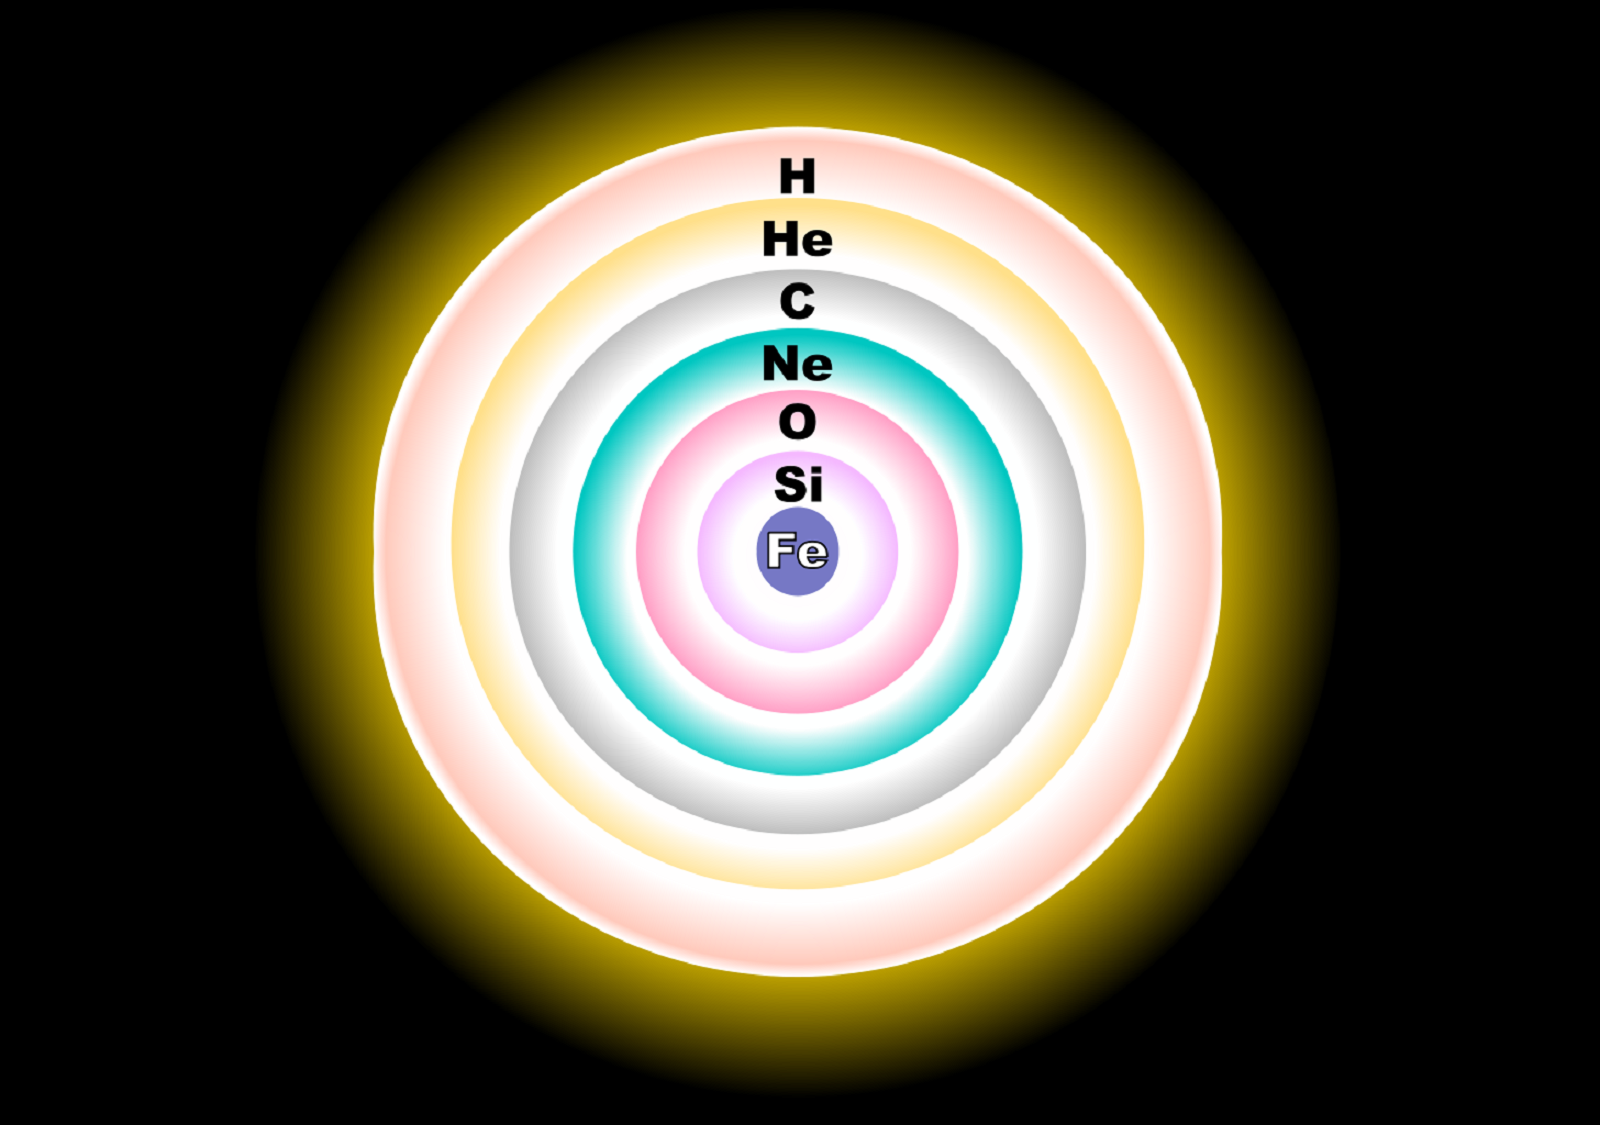
\includegraphics[scale=.25]{images/sncore}
\caption{Esquema no a escala de la estructura de una estrella masiva previo a su explosi\'on como supernova. Los elementos m\'as pesados se alojan en el centro, mientras que  los m\'as livianos, como el hidr\'ogeno o el helio lo hacen en la capa m\'as externa. \textit{Imagen publicada por R. J. Hall en WikiMedia Commons, 15 de agosto de 2007.}}
\label{fig:f0}
\end{figure}


Debido al aumento de temperatura, los electrones del n\'ucleo adquieren energ\'ia cin\'etica suficiente para escapar, desapareciendo as\'i la presi\'on que ejerc\'ian hacia el exterior. Finalmente el n\'ucleo colapsa liberando energ\'ia gravitacional y con ella las capas m\'as externas de la estrella son expulsadas en una gran explosi\'on. Este fen\'omeno se denomina \textit{supernova} e implica un aumento repentino del brillo de una estrella, incrementando su brillo en un factor de $10^8$ veces, pudiendo incluso ser m\'as brillante que la galaxia que la alberga.
\bigskip

En general la variaci\'on de la luminosidad de una supernova corresponde a una curva que crece r\'apidamente los primeros d\'ias (u horas), alcanzando un m\'aximo, para luego decaer. Cabe destacar que existen otros tipos de supernova, c\'omo las de las de tipo Ia y corresponden a otro fen\'omeno en donde participa una clase de estrella denominada enana blanca junto a otra estrella de cualquier otro tipo. La primera, al poseer una gravedad tan alta en su superficie es capaz de tomar material de su compa\~nera con lo que al superar las 1.44 $M_{\odot}$ se desencadenar\'ia la explosi\'on de supernova. 
\bigskip

Las supernovas de tipo Ia presentan un decaimiento casi continuo una vez alcanzado el m\'aximo, mientras que las de tipo II presentan dos ca\'idas: una inmediatamente despu\'es de su m\'aximo y otra una vez finalizado un per\'iodo de decaimiento suavizado (figura ~\ref{fig:f1}). Otra forma de diferenciarlas es la presencia de trazas de hidr\'ogeno en los espectros de \'estas: las supernovas de tipo Ia pr\'acticamente no presentan hidr\'ogeno (l\'ineas de absorci\'on distintivas) a diferencia de las de tipo II.\bigskip

\begin{figure}[h!]
\centering
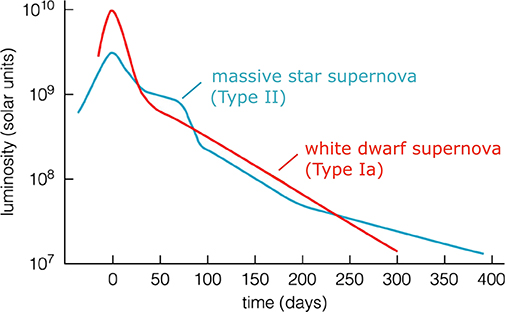
\includegraphics[scale=.8]{images/clear}
\caption{Curvas t\'ipicas de supernovas Ia (enana blanca) y II (estrella masiva). \textit{\textcopyright 2004 Pearson Education Inc., publishing as Addison-Wesley The Bizarre Stellar Graveyard.}}
\label{fig:f1}
\end{figure}


\section{High Cadence Transient Survey: HiTS}

El High Cadence Transient Survey\cite{hits} (desde ahora, HiTS) es un survey cuyo objetivo principal es detectar y seguir fen\'omenos transitorios estelares en escalas de tiempo que van desde horas a d\'ias, con especial atenci\'on a fases tempranas de explosiones de supernovas (primeras horas): el objetivo original de HiTS corresponde a la detecci\'on de un fen\'omeno llamado \textit{shock breakout} (SBO), un fen\'omeno que ocurre inmediatamente despu\'es del colapso del n\'ucleo de una estrella roja supergigante (una de las posibles etapas finales de una estrella masiva antes de \textit{explotar} en supernova II). Ver figura \ref{fig:f2}\footnote{$L_{\odot}= 3.828 \times 10^{26}$ W}.

%\ref{fig:f2}\footnote{\url{https://www.nasa.gov/feature/ames/Kepler/caught-for-the-first-time-the-early-flash-of-an-exploding-star}}


\begin{figure}[h!]
\centering
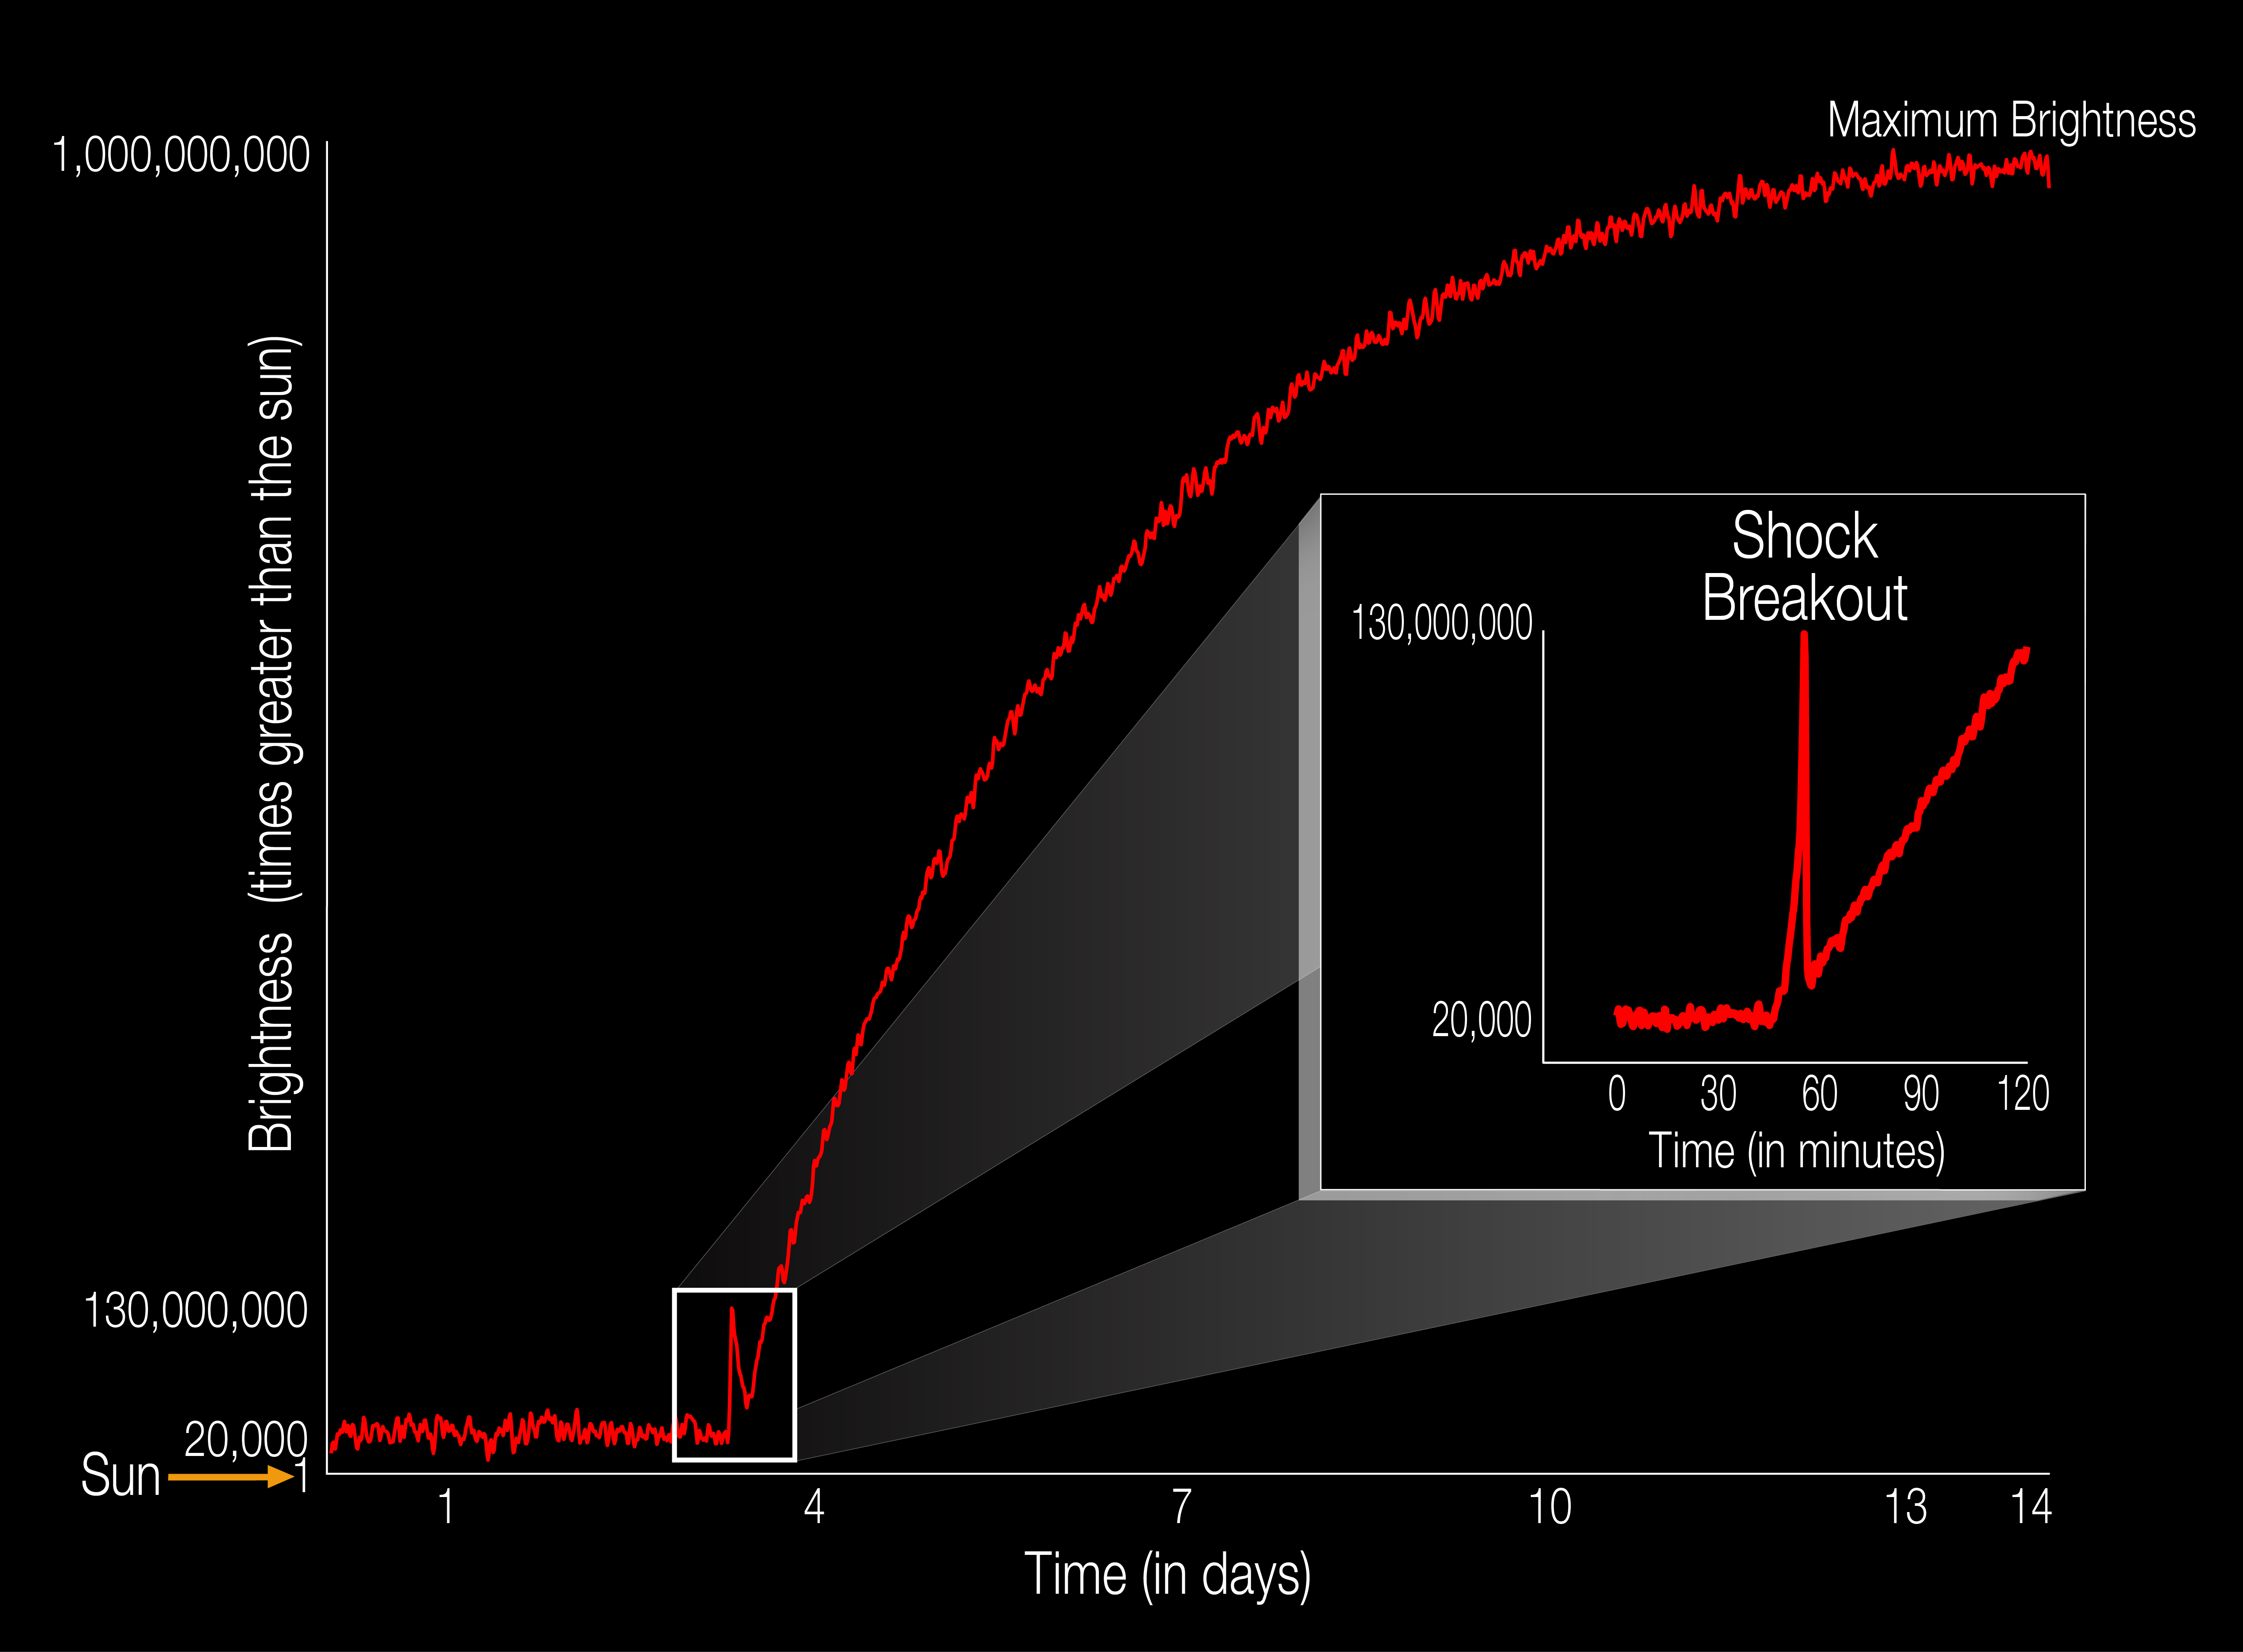
\includegraphics[scale=.25]{images/breakout}
\caption{Diagrama que ilustra la evoluci\'on del brillo de una supernova en t\'erminos de luminosidad solar ($L_{\odot}$) durante d\'ias. Se resalta el fen\'omeno de \textit{shock-breakout} apenas comienza el incremento de la luminosidad de la supernova. Esta imagen fue publicada en la p\'agina de la NASA destacando la primera vez que un evento como este es \textit{capturado} en la banda visible (por el telescopio espacial Kepler). \textit{NASA Ames/W. Stenzel. 2016}}
\label{fig:f2}
\end{figure}

HiTS utiliza la Dark Energy Camera (DECam, figura \ref{fig:f3}) para la obtenci\'on de sus im\'agenes. Esta c\'amara se encuentra montada en el Telescopio Blanco del Observatorio de Cerro Tololo (CTIO) en la regi\'on de Coquimbo, Chile. Esta c\'amara posee 62 detectores CCD de $2048 \times 4096$ p\'ixeles para la obtenci\'on de im\'agenes cient\'ificas y otros 12 para la gu\'ia, alineamiento y enfoque (ver Figuras \ref{fig:f3} y \ref{fig:f4} d\'onde se muestra disposici\'on de las c\'amaras CCD en el telescopio). 
\bigskip

\begin{figure}[h!]
\centering
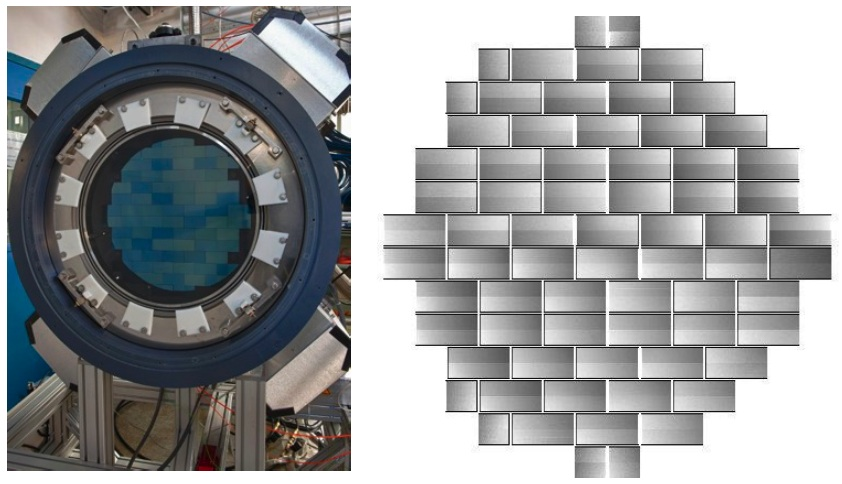
\includegraphics[scale=.5]{images/CCDs.jpg}
\caption{A la izquierda, estructura de la c\'amara DECam poblada con 62 chips CCDs. A la derecha, imagen \textit{flat field} desde DECam. \textit{Im\'agenes tomadas desde la p\'agina del Dark Energy Survey (\url{www.darkenergysurvey.org/the-des-project/instrument/the-camera}).}}
\label{fig:f3}
\end{figure}

Durante el proyecto HiTS se realizaron tres campa\~nas de observaci\'on en los a\~nos 2013, 2014 y 2015 durante el primer semestre de cada a\~no. Se escogieron 40 campos y 4 \'epocas por noche (tambi\'en por campo) para observaciones para el a\~no 2013 y en el 2014. Para la campa\~na del a\~no 2015 se escogieron 50 campos. En estas campa\~nas se obtuvieron m\'as de 120 candidatos a supernova. Sin embargo, no se logr\'o encontrar en estas rastros de SBO (figura \ref{fig:f2}) evento que comprendi\'o uno de los principales objetivos de HiTS. 

\begin{figure}[h!]
\centering
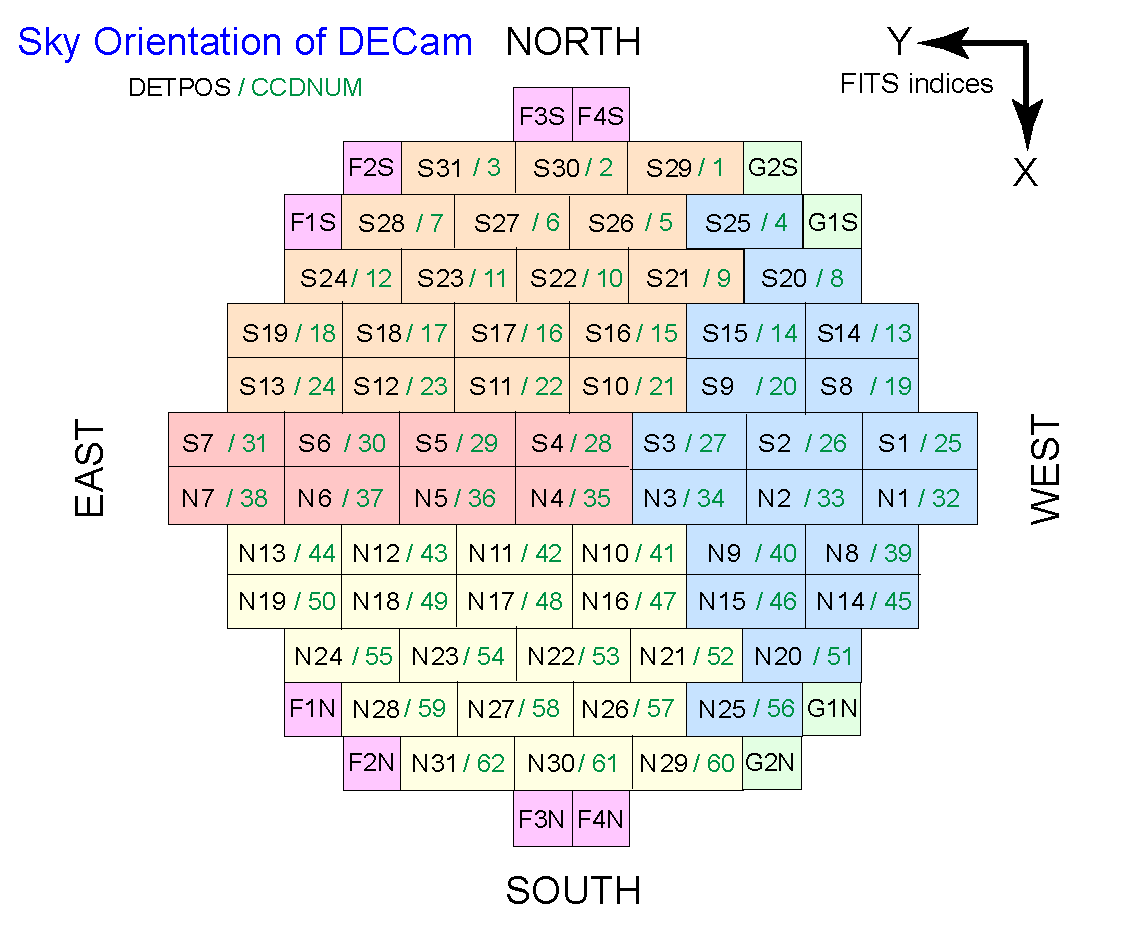
\includegraphics[scale=.75]{images/decam}
\caption{Orientaciones sobre el cielo y la huella espacial del arreglo de detectores en el plano focal. Se destacan los CCD cuya etiqueta comienzan con S o N, ya que estos corresponden a los detectores encargados de obtener las im\'agenes cient\'ificas. El etiquetado de estas componentes puede ser enga\~noso debido a que las iniciales de norte (North) y sur (South) est\'an invertidas en relaci\'on a la orientaci\'on del cielo. \textit{Imagen publicada en el sitio del CTIO (\url{http://www.ctio.noao.edu/noao/node/2250})}.}
\label{fig:f4}
\end{figure}

\begin{figure}
\centering
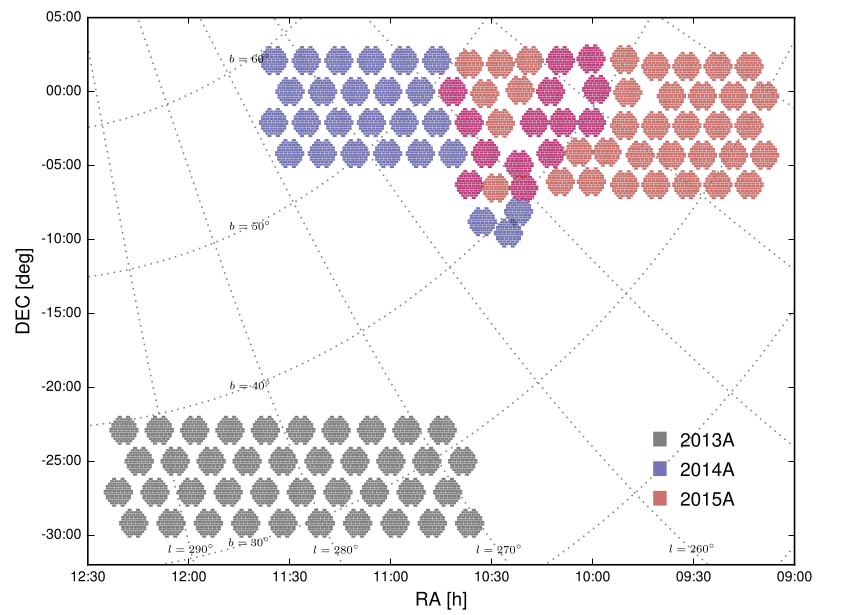
\includegraphics[scale=.5]{images/fields}
\caption{Distribuci\'on espacial de los campos observados durante los primeros semestres de los a\~nos 2013 (gris), 2014 (azul) y 2015 (naranjo). En tono rojo, los mismos campos del a\~no 2015 y 2014 (superposici\'on). \textit{F. F\"orster et al., 2015. HiTS real-time supernova detections.}}
\end{figure}

\subsection{Datos obtenidos durante el a\~no 2015}\label{ssec:data}
Como se mencion\'o anteriormente, la campa\~na del a\~no 2015 tuvo lugar el primer semestre de ese a\~no. El per\'iodo en que se llev\'o a cabo fue durante los meses de febrero y marzo; espec\'ificamente entre los d\'ias 17 de febrero a 14 de marzo.
\bigskip

El per\'iodo comprendido por los d\'ias 17 a 22 de febrero fue el de mayor latencia, obteni\'endose cinco \'epocas (observaciones) por noche por cada campo. Posteriormente la toma de observaciones cesa y se reanuda a partir del 24 de febrero con una latencia de a lo m\'as tres \'epocas por noche y campo con interrupciones de hasta diez d\'ias finalizando el 14 de marzo.

\section{El filtro de Kalman}
La evoluci\'on determin\'istica de un sistema f\'isico en el tiempo es conocida si el estado del sistema es medido con absoluta precisi\'on en cada instante de tiempo (i.e., en un entorno donde es posible despreciar fen\'omenos cu\'anticos). Sin embargo toda medici\'on est\'a sujeta a incertezas finitas. Para sistemas los cuales son observados entre intervalos prolongados de tiempo, se prevee que las diferencias entre los estados estimados y los medidos se incrementen con el tiempo. Para la obtenci\'on de predicciones lo m\'as confiables posible se requiere que el sistema sea regularmente monitoreado y sus estados estimados puedan ser considerados confiables en un lapso de tiempo apropiado. 
\bigskip

Los filtros de Kalman son m\'etodos que proveen un compromiso (o trade-off) entre los valores esperados del estado actual de un sistema y las mediciones que proporcionan informaci\'on de su estado real. La aplicaci\'on de un filtro de Kalman est\'a pensada como un proceso de dos fases:
\begin{enumerate}
\item \textbf{Fase predictiva:} Una estimaci\'on del estado actual del sistema que se basa en la estimaci\'on del estado previo o \'ultimo estado. Esta predicci\'on se denomina usualmente como estado estimado \textit{a priori}. 
\item \textbf{Fase correctiva:} La estimaci\'on del estado \textit{a priori} es corregida con una medida actual para refinar la aproximaci\'on. Esta mejora se denomina \textit{aproximaci\'on a posteriori.}
\end{enumerate}

T\'ipicamente estas fases de predicci\'on y correcci\'on se van alternando mientras se estudia el comportamiento f\'isico de alg\'un sistema.
\bigskip

\subsection{Filtro de Kalman B\'asico}
El filtro de Kalman B\'asico \cite{kalman} asume un comportamiento de sistema lineal y que las mediciones y las predicciones siguen una distribuci\'on Gaussiana. 
\bigskip

A continuaci\'on se describen las componentes del desarrollo matem\'atico del filtro:

\begin{itemize}
\item \textbf{$F_k$:} Matriz de transici\'on de estado, de dimensiones $N\times N$ (N es el n\'umero de variables de estado).
\item \textbf{$H_k$:} Matriz de transformaci\'on de estado a medici\'on, $K\times N$ (K corresponde a las mediciones realizadas en un instante k de una variable de estado).
\item \textbf{$Q_k$:} Matriz de covarianza del ruido del proceso ($N\times N$).
\item \textbf{$R_k$:} Matriz de covarianza del ruido de las mediciones ($K\times K$).
\item \textbf{$B_k$:} Matriz de control de entrada (contiene alteraciones que se querr\'ian agregar al sistema de manera deliberada, por ejemplo, como la condici\'on de parada de un veh\'iculo en movimiento). Esta matriz es de dimensiones $N\times L$, donde $L$ es la dimensi\'on del vector de control de entrada $u_k$.
\end{itemize}
\bigskip
Se har\'a uso de la notaci\'on en sub\'indices $m|n$, en las estimaciones de estado y covarianzas, para explicitar el instante de tiempo al cual pertenecen:  $m$; y al instante de tiempo de donde se extrae la informaci\'on: $n$.
\bigskip

En el instante $k-1$, se obtienen dos cantidades 
\begin{itemize}
\item $\hat{x}_{k|k-1}$ : Estado estimado \textit{a priori} (vector de dimensi\'on $N$). 
\item $P_{k|k-1}$ : Matriz de covarianza \textit{a priori} (matriz de dimensi\'on $N\times N$ ).
\end{itemize}
\bigskip

Luego, en la fase de correcci\'on se calculan:

\begin{itemize}
\item $\hat{z}_k$ : Predicci\'on de la medida.
\item $\tilde{z}_k$ : Residuo de la diferencia entre la medici\'on real, $z_k$, y su predicci\'on, $\hat{z}_k$.
\item $\hat{x}_{k|k}$ : Estado estimado \textit{a posteriori}.
\item $P_{k|k}$ : Matriz de covarianza \textit{a posteriori}.
\end{itemize}
\bigskip

Con estas variables, podemos describir las Ecuaciones que explican la evoluci\'on del proceso del algoritmo de Kalman b\'asico (un esquema de los c\'alculos involucrados en el proceso de estimaci\'on de estados se puede ver en la figura \ref{fig:kfb}):
\begin{enumerate}
\item \textbf{Fase predictiva:}\\
Las ecuaciones de estimaci\'on de estado y matriz de covarianza \textit{a priori} son:
\begin{equation}
\hat{x}_{k|k-1} = F_k \hat{x}_{k-1|k-1} + B_k u_k,
\label{eq:eq1}
\end{equation}
\begin{equation}
P_{k|k-1} = F_{k}P_{k-1|k-1}F_k^{T} + Q_k. 
\label{eq:eq2}
\end{equation}
\item \textbf{Fase correctiva:}\\
Las ecuaciones de stimaci\'on de estado y matriz de covarianza \textit{a posteriori} son:
\begin{equation}
\hat{z}_k = H_{k} \hat{x}_{k|k-1},
\label{eq:eq3}
\end{equation}
\begin{equation}
\tilde{z}_k=z_k - \hat{z}_k.
\label{eq:eq4}
\end{equation}
La Ecuaci\'on \ref{eq:eq4} describe la obtenci\'on de un residuo de la diferencia entre la predicci\'on y la medida $z_k$. Posteriormente se calcula la matriz de covarianza entre residuos ($S_k$), con la que se calcula la ganancia de Kalman: $K_k$ . Formalmente,
\begin{equation}
S_k = H_k P_{k|k-1} H_{k}^T + R_k,
\label{eq:eq5}
\end{equation}
\begin{equation}
K_k = P_{k|k-1} H_k^T S_k^{-1}.
\label{eq:eq6}
\end{equation}
Con la ganancia de Kalman calculada, se actualiza el valor de la estimaci\'on de estado (\ref{eq:eq7}) y la matriz de covarianza a posteriori (Ecuaci\'on \ref{eq:eq8}), del siguiente modo, 

\begin{equation}
\hat{x}_{k|k} = \hat{x}_{k|k-1} + K_k \tilde{z}_k,
\label{eq:eq7}
\end{equation}

\begin{equation}
P_{k|k} = (I_N - K_kH_k)P_{k|k-1}.
\label{eq:eq8}
\end{equation}
\bigskip

\end{enumerate}
La figura \ref{fig:kfb} resume el proceso de predicci\'on (obtenci\'on de las cantidades a priori, $\hat{x}_{k|k-1}$ y $P_{k|k-1}$) y correcci\'on (generaci\'on de las estimaciones, $\hat{x}_{k+1|k}$ y $P_{k+1|k}$, a partir de las cantidades a posteriori  $\hat{x}_{k|k}$ y $P_{k|k}$) del filtro de Kalman B\'asico. 
\begin{figure}[h!]
\centering
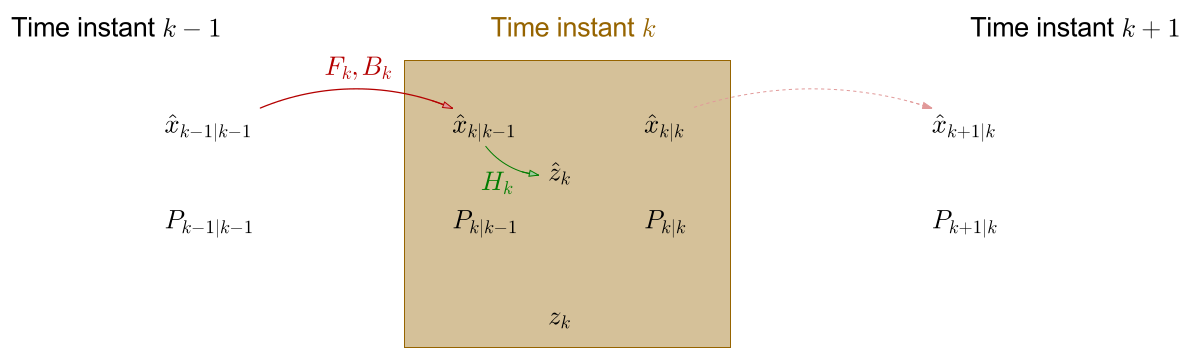
\includegraphics[scale=0.5]{images/kfb}
\caption{Representaci\'on del proceso de predicci\'on (obtenci\'on de cantidades a priori) de las cantidades $\hat{x}_{k|k-1}$ y $P_{k|k-1}$;  y de correcci\'on (estimaci\'on a posteriori) para obtener las cantidades $\hat{x}_{k+1|k}$ y $P_{k+1|k}$. \textit{E. Matsinos, 2016. The Kalman Filter: a didactical overview.}}
\label{fig:kfb}
\end{figure}

\subsection{Filtro de Kalman de M\'axima Correntrop\'ia}

El filtro de Kalman basado en m\'axima correntrop\'ia \cite{badong}, difiere del filtro de Kalman tradicional (b\'asico) en que no asume gaussianidad en las observaciones, considerando casos en que una se\~nal puede ser perturbada por pulsos de ruido que sigan una distribuci\'on de cola pesada. En esta oportunidad se utiliza el \textit{criterio de m\'axima correntrop\'ia} para el proceso de correcci\'on. 
\bigskip

La correntrop\'ia es una medida de similitud entre dos variables aleatorias. Supongamos, $X,Y \in \mathbb{R}$ con una distribuci\'on conjunta $F_{XY} (x,y)$. Definimos la correntrop\'ia matem\'aticamente como:

\begin{equation}
V(X,Y) = E[\kappa(X,Y)] = \int \kappa(x,y) dF_{XY} (x,y),
\label{eq:eqcorr}
\end{equation}
\noindent
donde $E$ representa al operador de esperanza y $\kappa(,)$ corresponde a un kernel Mercer invariante a desplazamientos (teorema de Mercer, \cite{mercer}). Para este filtro se emplea una funci\'on de kernel Gaussiana, dado por

\begin{equation}
\kappa(x, y) = G_{\sigma} (e) = exp \left(-\dfrac{e^2}{2\sigma^2} \right).
\label{eq:eqkappa}
\end{equation}

La \textit{funci\'on de costo} de m\'axima correntrop\'ia se define como:
\begin{equation}
J_{MCC} = \dfrac{1}{N} \sum_{i=1}^N G_{\sigma} (e (i)).
\label{eq:costo}
\end{equation}
La Ecuaci\'on \ref{eq:costo} representa la funci\'on a maximizar, la que calcula la estimaci\'on corregida para el estado en el instante $k$,

\begin{equation}
\hat{x}_k = arg max_{x} (J_{MCC})= argmax_x (\sum_{i=1} G_{\sigma} (e_i(k))).
\label{eq:max}
\end{equation}
\bigskip

Para obtener el m\'aximo de correntrop\'ia se procede a calcular el error residual $\tilde{e}_i$ estimado como,

\begin{equation}
\tilde{e}_i = d_{i,k} - w_{i,k} \hat{x}_{t-1, k|k}.
\label{eq:eq9}
\end{equation}

Con estos residuos definimos las matrices diagonales, descritas en las Ecuaciones siguientes: 
\bigskip

\begin{equation}
\tilde{C_{x, k}}= diag(G_{\sigma}(\tilde{e}_{1, k}),..., G_{\sigma}(\tilde{e}_{n, k})),
\label{eq:eq10}
\end{equation}

\begin{equation}
\tilde{C_{y, k}}= diag(G_{\sigma}(\tilde{e}_{n+1, k}),..., G_{\sigma}(\tilde{e}_{n+m, k})).
\label{eq:eq11}
\end{equation}

La matriz \ref{eq:eq10} corresponde a evaluaciones del kernel en errores estimados de predicci\'on y la matriz \ref{eq:eq11} en errores propios de las observaciones (ruido). Luego se realiza una transformaci\'on de la covarianza del ruido de las mediciones usando una descomposici\'on de Choleski ($B_{r, k}$) en el instante $k$ \cite{chen}, seg\'un la expresi\'on:
\bigskip
 
\begin{equation}
\tilde{R}_k = B_{r, k} \tilde{C}_{y, k}^{-1}B_{r, k|k-1}^T.
\label{eq:eq12}
\end{equation}

Luego se calcula la transformaci\'on de la predicci\'on de la matriz de covarianza de las estimaciones de estado, $P_{k|k-1}$,
\begin{equation}
\tilde{P}_{k|k-1} = B_{p, k|k-1} \tilde{C}_{x, k}^{-1}B_{p, k|k-1}^T.
\label{eq:eq13}
\end{equation}

Posteriormente se calcula la ganancia de Kalman para este nuevo sistema,
\begin{equation}
\tilde{K} = \tilde{P}_{k|k-1} H_k^T (H_k \tilde{P}_{k|k-1} H_k^T + \tilde{R}_k)^{-1}. 
\label{eq:eq14}
\end{equation}

Finalmente la actualizaci\'on de la estimaci\'on de estado para el instante $k$ queda como: 
\begin{equation}
\hat{x}_{t, k|k} = \hat{x}_{k|k-1} + \tilde{K}_{k} (y_k - H_k \hat{x}_{k|k-1}).
\label{eq:eq15}
\end{equation}
\bigskip

Las Ecuaciones \ref{eq:eq9} a \ref{eq:eq15} se repiten secuencialmente hasta satisfacer la condici\'on:

\begin{equation}
\dfrac{\parallel  \hat{x}_{t, k|k} - \hat{x}_{t-1, k|k} \parallel }{\parallel \hat{x}_{t-1, k|k} \parallel} \leq \epsilon.
\label{eq:eq16}
\end{equation}

El valor de $\epsilon$ es definido por el usuario y corresponde a un criterio de detenci\'on (el algoritmo tambi\'en puede detenerse definiendo un m\'aximo de n\'umero de pasos). Finalmente se calcula la matriz de covarianza para el instante actual, $k$.
%\item \textbf{C\'alculo de la m\'axima correntrop\'ia basado en funci\'on costo}
\begin{equation}
P_{k|k} = \left(I - \tilde{K}_kH_k \right)P_{k|k-1} \left(I - \tilde{K}_k H_k \right)^T + \tilde{K}_kR_k\tilde{K}^T_k.
\label{eq:eq17}
\end{equation}

\subsection{Filtro de Kalman Unscented (UKF)}
\label{ssec:ukf}
Este filtro corresponde a aquel que se pretende agregar a la familia de filtros ya desarrollada en el programa base.
\bigskip

\begin{enumerate}
\item \textbf{Fase predictiva:}\\
En esta versi\'on del filtro \cite{ukf} ya no se habla de matrices de transici\'on de estado, $F_k$, ni de matrices de transformaci\'on de estado-a-medici\'on, $H_k$, sino m\'as bien de funciones diferenciables $f$ y $h$ respectivamente para describir la transici\'on de estados  y la transformaci\'on de estos a estimaciones a priori. Sin embargo, previo a estas transiciones se deben seleccionar 2N+1 puntos representativos alrededor de $\hat{x}_{k-1|k-1}$ y evaluar estos en la funci\'on no lineal $f$, para obtener las estimaciones de $\hat{x}_{k|k-1}$ y $P_{k|k-1}$. Estos puntos se conocen como \textit{puntos sigma} (en la Figura \ref{fig:fukf} se visualiza el proceso de predicci\'on al momento de obtener el primer conjunto de \textit{puntos sigma}, propagarlos usando la funci\'on $f$ y obtener $\hat{x}_{k|k-1}$ y $P_{k|k-1}$, es decir, la matriz de estados y de covarianza \textit{a priori}). 

\begin{figure}[h!]
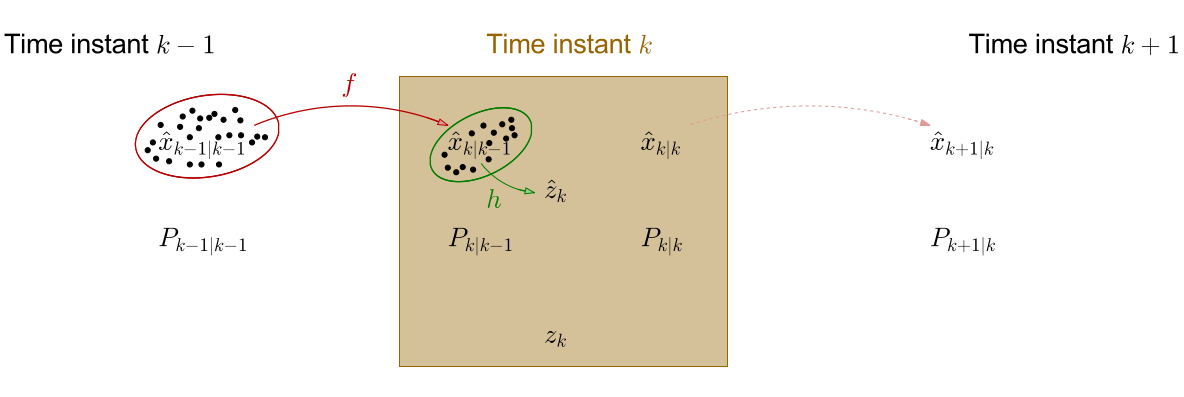
\includegraphics[scale=.5]{images/ukf}
\caption{Representaci\'on del funcionamiento del filtro UKF. En esta oportunidad se hace uso de la funci\'on $f$ y $h$ para obtener las transformaciones $x_{k-1}\rightarrow x_k$ y $x_{k}\rightarrow z_k$. Esto se logra con la evaluaci\'on de los 2N+1 \textit{puntos sigma} generados durante la etapa de predicci\'on (y posteriormente en la etapa de correcci\'on). \textit{E. Matsinos, 2016. The Kalman Filter: a didactical overview.}}
\label{fig:fukf} 
\end{figure}

La generaci\'on de los 2N+1 puntos, se realiza a partir de la \'ultima estimaci\'on $\hat{x}_{k-1|k-1}$  de la siguiente forma:
\begin{equation}
\label{eq:eq18}
\begin{gathered}
\bar{x}_{k-1| k-1}^0 = \hat{x}_{k-1|k-1}\\
\bar{x}_{k-1| k-1}^0 = \hat{x}_{k-1|k-1}+ \chi_i, \quad  \forall i \in [1, N]\\
\bar{x}_{k-1| k-1}^0 = \hat{x}_{k-1|k-1}- \chi_{i-N}, \quad  \forall i \in [N+1, 2N]
\end{gathered},
\end{equation}
donde la cantidad $\chi_i$ corresponde a la i-\'esima columna de la \textit{ra\'iz cuadrada} de la matriz:

 \begin{equation}
 (N+\lambda) P_{k-1 | k-1}.
 \label{eq:eq19}
 \end{equation}
La matriz (\ref{eq:eq19}) puede obtenerse a partir de la descomposic\'on de Choleski. Por otro lado los puntos sigma se generan junto a dos conjuntos de pesos: $\lbrace w_x^{i} \rbrace$ y $\lbrace w_p^{i} \rbrace$. El primer conjunto se emplea en la estimaci\'on del estado y la predicci\'on de la medida, mientras que el segundo conjunto es usado para obtener las matrices de covarianza. Estos pesos son definidos como:
\begin{equation}
\label{eq:eq20}
\begin{gathered}
w^0_x = \dfrac{\lambda}{N+\lambda}\\
w^0_p = w^0_x + 1 - \alpha^2 + \beta\\
w^i_x = w^i_p = \dfrac{1}{2(N+\lambda)}\\
\sum_i^{2N} w^i_x = 1
\end{gathered}.
\end{equation}
De \ref{eq:eq20} se desprende que los pesos $w_x^i$ son normalizados. Por otro lado, el par\'ametro $\lambda$ se puede escribir en t\'erminos de los valores de $\alpha \in \left( 0,1\right]$ y $\kappa$ seg\'un la expresi\'on siguiente:%\ref{eq:eq21}

\begin{equation}
\label{eq:eq21}
\lambda = \alpha^2  (N + \kappa)- N.
\end{equation}

Los par\'ametros $\alpha$, $\beta$ y $\kappa$ deben ser ajustados acorde al problema que se est\'a estudiando.
\bigskip

Con esto, es posible escribir las Ecuaciones de la fase predictiva.
\begin{itemize}
\item Estimaci\'on a priori de los estados. La ecuaci\'on correspondiente es:\\
\begin{equation}
\label{eq:eq22}
\hat{x}_{k|k-1} = \sum_{i=0}^{2N} w_{x}^i f(\bar{x}^i_{k-1|k-1}).
\end{equation}

\item Estimaci\'on a priori de la matriz de covarianza. La ecuaci\'on correspondiente es:\\

\begin{equation}
\label{eq:eq23}
P_{k|k-1} = \sum_{i=0}^{2N} w_p^i \left( f(\bar{x}^i_{k-1|k-1})  - \hat{x}_{k|k-1}\right)\left( f(\bar{x}^i_{k-1|k-1}) - \hat{x}_{k|k-1}  \right)^T + Q_k.
\end{equation}
\end{itemize}


\item \textbf{Fase correctiva:}\\
Durante la fase de correcci\'on, nuevamente se seleccionan 2N+1 puntos representativos, alrededor de $\hat{x}_{k|k-1}$. Estos posteriormente son evaluados en la funci\'on no-linear $h$.

\begin{equation}
\label{eq:eq24}
\begin{gathered}
\bar{y}_{k-1| k-1}^0 = \hat{x}_{k|k-1}\\
\bar{y}_{k-1| k-1}^i = \hat{x}_{k|k-1}+ \psi_i, \quad  \forall i \in [1, N]\\
\bar{y}_{k-1| k-1}^i = \hat{x}_{k|k-1}- \psi_{i-N}, \quad  \forall i \in [N+1, 2N].\\
\end{gathered}
\end{equation}
La cantidad $\psi_i$ representa la i-\'esima columna de la matriz de \textit{ra\'iz cuadrada} $(N+\lambda)P_{k|k-1}$.

Las Ecuaciones del proceso de correcci\'on, por tanto, quedan como sigue:
\begin{itemize}
\item Predicci\'on de las medidas:\\
\begin{equation}
\label{eq:eq25}
\hat{z}_{k} = \sum_{i=0}^{2N} w_x^i h(y_{k|k-1}^{-i}).
\end{equation}
\item Los residuos de las mediciones pueden obtenerse como:\\
\begin{equation}
\tilde{z}_k = z_k - \hat{z}_k.
\label{eq:eq26}
\end{equation}
\item La matriz de innovaci\'on:\\
\begin{equation}
S_k = \sum_{i=0}^{2N} w_p^i (h(y_{k|k-1}^{-i}) - \hat{z}_k)(h(y_{k|k-1}^{-i})^T + R_k.
\label{eq:eq27}
\end{equation}
\item La matriz de covarianza cruzada de estado a medida se describe como:\\
\begin{equation}
C_k = \sum_{i=0}^{2N} w_p^i ( f(\bar{x}^i_{k-1 | k-1})- \hat{x}_{k|k-1} )( h(y_{k|k-1}^{-i}) - \hat{z}_k )^T.
\label{eq:eq28}
\end{equation}
\item La ganancia \'optima finalmente queda:\\
\begin{equation}
K_k = C_kS_k^{-1}.
\label{eq:eq29}
\end{equation}
\item La estimaci\'on \textit{a posteriori} de estado:\\
\begin{equation}
\label{eq:eq30}
 \hat{x}_{k|k} =  \hat{x}_{k|k-1} + K_k \tilde{z}.
\end{equation}
\item Por otro lado, la ecuaci\'on para la matriz de covarianza:\\
\begin{equation}
\label{eq:eq31}
P_{k|k} = P_{k|k-1} - K_kS_kK_k^T.
\end{equation}
\end{itemize}
Los pesos $w_x^i$ y $w_p^i$ son los mismos calculados en la expresi\'on \ref{eq:eq20}, de la fase de predicci\'on.
\end{enumerate}

\section{Laboratorio Nacional de Computaci\'on de Alto Desempe\~no (NLHPC)}
El National Laboratory for High Performance Computing (NLHPC) es un proyecto asociativo, financiado por el PIA de CONICYT el cual dispone de un potente sistema computacional que est\'a disponible a la comunidad cient\'ifica y acad\'emica nacional (instituciones de investigaci\'on, industria y universidades), estimulando su uso en el desarrollo de \'areas de investigaci\'on que requieran de herramientas computacionales robustas que deban ser usadas de manera intensiva. 
\bigskip

Para la realizaci\'on de esta tesis se hizo uso de uno de los nodos del cl\'uster de Leftraru, el supercomputador del NLHPC disponible para la comunidad investigadora desde el 2014 en las instalaciones del Centro de Modelamiento Matem\'atico (CMM) de la Universidad de Chile.  

\begin{itemize}
\item 132 nodos de c\'omputo HP (128 nodos HP SL230 y 4 nodos HP SL250), cada uno con dos procesadores de 10 cores Intel Xeon Ivy Bridge E5-2660 V2.
\item 2640 n\'ucleos
\item 6.25 TB de RAM
\item 274TB de almacenamiento Lustre (DDN EXAScaler)
\item 12 co-procesadores Intel Xeon Phi5110p de 2 TFlops
\item Capacidad de c\'omputo de 70 TFlops 
\end{itemize} 

Para la ejecuci\'on de las pruebas se emplearon cuatro cores, 2400 MB por cada CPU (m\'axima RAM permitida) y un \textit{job-array} de largo 93.

